\documentclass[a4,center,fleqn]{NAR}

% Enter dates of publication
\copyrightyear{2008}
\pubdate{31 July 2009}
\pubyear{2009}
\jvolume{37}
\jissue{12}

%\articlesubtype{This is the article type (optional)}
\usepackage{lscape}
\usepackage{threeparttable}
\usepackage{booktabs}
\usepackage[bottom]{footmisc}


\begin{document}

\title{Review on Rare Variant Detection Methods for Cell-free DNA Next-generation Sequencing Data}

\author{%
Fan Zhang\,$^{1}$
and Patrick Flaherty\,$^{1, 2}$
\footnote{To whom correspondence should be addressed.
Tel: 413-545-1796; Fax: 413-545-1801; Email: flaherty@math.umass.edu}}



\address{%
$^{1}$Department of Biomedical Engineering, Worcester Polytechnic Institute, MA, USA
and
$^{2}$Department of Mathematics and Statistics, University of Massachusetts, Amherst, MA, USA}
% Affiliation must include:
% Department name, institution name, full road and district address,
% state, Zip or postal code, country

\history{%
Received January 1, 2009;
Revised February 1, 2009;
Accepted March 1, 2009}

\maketitle

\begin{abstract}
Next-generation sequencing enables the generation of thousands of millions of short reads parallely to reveal genomic heterogeneity in disease samples like cancer.
Targeting this sequencing power towards cell-free DNA enables the technology to be used for prenatal diagnostics, cancer monitoring, and transplant monitoring.
Many statistical or computational methods have been developed to detect single nucleotide variants in mixed samples, but precise detection of rare single nucleotide variants is still a major challenge.
Here, we review the progress the community has made in recent years in terms of resolution, sensitivity, specificity, and computational time.
%Even though several methods are proposed to detect very rare variants in the heterogeneous samples, each method has its bias or is only designed for a particular application of interest.
%In this review, we highlight the need for sensitive variant detection methods for cell-free DNA data and discuss the hallmarks of a good statistical method from the perspective of accuracy, scalability, and robustness.
%In this review, we highlight the need for sensitive variant detection methods for cell-free DNA sequencing data.
%We list the issues, quality control, depth of coverage, sequencing errors, and sample size, and discuss how these factors impact on the power of variant detection methods.
We outline the statistical and computational metrics that are used to evaluate statistical rare variant detection methods and survey 30 methods for rare variant detection.
Finally, future challenges and opportunities are addressed.

\end{abstract}


\section{Introduction}
%\subsection{Sequence Analysis Pipeline}
%Scope of the article: nucleotides and variant calling in the context of larger pipeline.
Next-generation sequencing (NGS) technology has revealed the presence of extensive genomic variants in clinical samples~\citep{koboldt2013next}.
The Cancer Genome Atlas (TCGA) provides a large number of cancer genomic data sets for characterization of cancer-specific variant profiles~\citep{cancer2012comprehensive}.
In general, genomic variants can be present in the form of single nucleotide variants (SNVs), insertions and deletions, structural variants, and copy number variations~\citep{Bao2014}.
Single nucleotide variant is a primary source of genetic variation that can cause susceptibility to disease or drug resistance to anti-tumour therapeutics~\citep{kessler2014resistance}.
The general pipeline to analyze single nucleotide variants in the large-scale NGS data basically consists five main steps: quality control, preprocessing, alignment, post-alignment processing, and variant analysis~\citep{pabinger2014survey, Bao2014}.
Variant analysis basically contains three main parts: variant detection, annotation, and visualization, among which variant detection is crucial for NGS data analysis with an objective of discovering disease-causing variants.


%Detection in cell free DNA using NGS 
Cell-free DNA (cfDNA) next-generation sequencing has been performed to accurately detect genetic variants that can be used as biomarkers for early cancer detection and anti-cancer treatment monitoring~\citep{schwarzenbach2011cell, zhou2014pilot}.
It has been demonstrated that cfDNA sequencing is able to detect tumour-derived variants with high sensitivity and specificity in the frequently mutated genes in pancreatobiliary tumour samples~\citep{zill2015cell}.
However, it is an challenge to detect variants in cfDNA due to the low allele frequency of the variants in tumour samples.
Another reason is the low fraction of cfDNA and the dilution effect of the normal DNA in the blood. 
Thus, bioinformatics methods for cfDNA sequencing analysis are more than desirable to analyze and interpret the rare variants that are relevant to cancer diagnostic and prognostic.


%Outline the paper here with one paragraph overview per section.
In this review, we focus on single nucleotide variant detection in cfDNA next-generation sequencing data and classification of current computational and statistical variant detection methods.
We first describe the flowchart of variant detection in NGS cfDNA data and then highlight the necessity of sensitive variant detection methods from the perspective of biological impacts and statistical accuracy.
We also consider the hallmarks of a good variant detection method based on the evaluation of accuracy, scalability, and robustness.
Furthermore, we discuss the issues that will effect the ability of variant detection methods.
Finally, we classify the state-of-the-art variant detection methods into the categories of probabilistic and non-probabilistic methods and outline each method in detail.
An overall framework of developing Bayesian-based method for variant detection is described as well.
In conclusion, we discuss the challenges and opportunities of statistical methods for variant detection for the future.

\clearpage

\section{Variant detection in cell-free DNA sequencing data}

NGS of cfDNA is a non-invasive method for tumour-associated or drug resistant variants detection, which will be highly promising for detecting clinical biomarkers. 
Many remarkable variants on tumour-specific genes, such as \textit{TP53}, \textit{BRAF}, and \textit{KRAS}, can be observed on cfDNA.
\textit{BRAF} variant V600E was first detected on cfDNA by~\citep{shinozaki2007utility} at different stages and its clinical use for monitoring behavior of melanoma patients was demonstrated.
A "liquid biopsy" method is used to identify variants at allele frequency of $2\%$ with high sensitivity and specificity in the circulating cfDNA of tumours~\citep{forshew2012noninvasive}.
NGS technology also enabled fetal DNA sequencing in maternal plasma.
A NGS-based cfDNA sequencing with $65\times$ coverage revealed genome-wide variants of the fetus and demonstrated different patterns of fetal and maternal genomes~\citep{lo2010maternal}.

We summarize a workflow for variant detection in cfDNA NGS data in Figure \ref{fig:flowchart}.
CfDNA is first extracted from plasma where tumour cfDNA (blue curves) and normal cfDNA (green curves) are mixed together.
After library construction and sequencing process, reads are aligned to the reference genome to prepare for alteration detection.
Then, a rare variant detection method is applied to identify single nucleotide variants in the cfDNA sequencing data.
Finally, tumour-associated variants are obtained and can be further interpreted for clinical utility.
These clinically relevant variants can be considered as candidate biomarkers and identification of these variants are required to monitor response to treatment.


\begin{figure*}[ht]
\centering
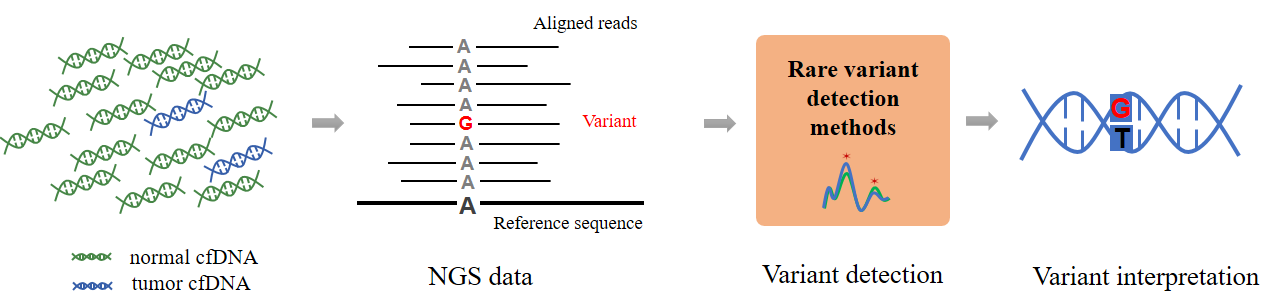
\includegraphics[width=1\textwidth]{flowchart.png}
\caption{Flowchart of variant detection in cfDNA from NGS data.}
\label{fig:flowchart}
\end{figure*}


\section{Why do we need a sensitive variant detection method?}

\subsection{Biological impacts}

The cost of whole-genome sequence (WGS) or whole-exome sequence (WES) has been reduced to below $\$1,000$ ~\citep{caulfield2013reflections}, which has made it possible to have a deeper understanding of the structure of genomes to improve the effectiveness of disease treatment. 
Most variants revealed by the WGS and WES are demonstrated to be rare by The 1000 Genomes Project Consortium~\citep{10002010map} and rare variants do cause risk of disease or have large effects~\citep{koboldt2013next, kosmicki2016discovery, ng2010exome, keller2013mutations}.
Currently, the bottleneck of large-scale sequencing is accurate and efficient data analysis rather than data generation.
The oseltamivir resistance variant, H275Y, exists in a fraction of $0.18\%$ in a H1N1 clinical sample~\citep{Flaherty2012}.
However, deep sequencing of WGS or WES on multiple samples is so expensive that detection of a $0.1\%$ variant event is unfeasible.
Thus, accurate and sensitive variant detection methods are needed to identify this causal variant to improve the efficacy of antiviral therapy.
Recently, detection of variants in low fraction of cfDNA is effective and efficient in monitoring tumour progression, which will be a complement to the cancer tissue biopsies.
A pilot study has shown the feasibility of leukemic cfDNA in resolving DNA abnormalities~\citep{zhou2014pilot}.
Therefore, sensitive computational methods are needed to accelerate rare variants detection and interpretation in the cfDNA data in order to derive further biological inference.


\subsection{Statistical accuracy}

%Since the allele frequency of rare variants in the public genomes data is relatively low, it needs methods with high statistical power to identify rare variants in impure samples. 
Since rare variants in the public genomes data are relatively low in allele frequency, methods with high statistical power are needed.
It is difficult to guarantee statistical accuracy for variant detection in low or moderate sequencing read depths because simple strategies based on cut-offs for counting alleles may lead to wrong prediction.
To achieve high statistical accuracy, statistical and probabilistic methods have been appeared and mature in providing measures of uncertainty for genotypes inference in variant detection~\citep{Nielsen2011}.  
Specifically, Bayesian statistical methods are popular for developing sensitive variant detection tools by incorporating proper prior probabilities of possible genotypes and then predict the true genotype using a maximum a posteriori probability (MAP).
Several studies have used a binomial probabilistic distribution to model sequencing error distributions that can be further used to differentiate true biological variants from errors~\citep{Flaherty2012, Shiraishi2013, gerstung2012reliable, Christoforides2013}.
Thus, advanced statistical methods with high accuracy can be sensitive in detecting true rare variants by reducing the probability of causing false positives.

\section{Hallmarks of a good variant detection method}

\subsection{Accuracy}
Accurate detection of SNVs is essential because the detected variants that modulate chemotherapy resistance will help to find private novel variants in clinical cancer samples and suggest improved therapies.
Thus, accuracy is normally considered as the first criteria to evaluate the performance of variant detection methods.
To evaluate accuracy, simulated sequencing data sets can be used firstly to test variant detection methods since the underlying truth is known.
Benchmarking data sets, such as well-recognized sequencing samples, can also be performed to validate the methods if available.

Performance metrics are used to understand the basic values of true positive (TP), false positive (FP), true negative (TN), and false negative (FN).
A number of metrics have been chosen to assess accuracy, such as sensitivity, specificity, false positive rate, false discovery rate, accuracy and so on.
We list several common metrics for evaluating the accuracy of variant detection methods in Table \ref{tbl:metrics}.
Receiver operating characteristic (ROC) curves are very useful to visualize and interpret the performances of various methods as~\citep{Xu2014, Huang2015, He2015} did.
Since each metric has its uncertainty and is related to the sequence context, selection of desired metrics relies on specific purposes and a discussion about selecting metrics for accuracy evaluation is covered in detail in~\citep{Olson2015}.

Ideally, an accurate variant detection method should perform with high sensitivity, and specificity and low false discovery rate in identifying variants in a practical level of mutant allele frequencies.
Since it is impossible for statistical methods to acquire ideal accuracy in all circumstances, good variant detection methods should be capable to detect true variants to keep the false positive rate as low as possible in an acceptable accuracy for a particular data of interest.


\begin{table}[htp]
  \centering
  \footnotesize 
  \caption{Metrics for accuracy evaluation of variant detection methods.}\label{tbl:metrics}
  \begin{threeparttable}    
  \begin{tabular}{lll}
    \textbf{Metrics} & \textbf{Explanation} & \textbf{Derivation} \\
    \toprule    
    Sensitivity & true positive rate & $\frac{TP}{TP+FN}$ \\[0.2cm]
    Specificity & true negative rate & $\frac{TN}{FP+TN}$ \\[0.2cm]
    FPR   & false positive rate & $\frac{FP}{FP+TN}$ \\[0.2cm]
    FDR   & false discovery rate &  $\frac{FP}{FP+TP}$ \\[0.2cm]
    PPV   & positive predicted value or precision & $\frac{TP}{TP+FP}$ \\[0.2cm]
    NPV   & negative predicted value & $\frac{TN}{TN+FN}$ \\[0.2cm]
    ACC   & accuracy & $\frac{TP+TN}{TP+FP+TN+FN}$ \\[0.2cm]
    MCC   & Matthews correlation coefficient & $\frac{TP*TN-FP*FN}{\sqrt{P1*P2*N1*N2}}$ \\
    \bottomrule
    \end{tabular}%
    \begin{tablenotes}
	\item TP, true positive; FP, false positive; TN, true negative; FN, false negative;  
                 P1, TP+FP; P2, TP+FN; N1, TN+FP; N2, TN+FN.
    \end{tablenotes}
\end{threeparttable}
\end{table}



\subsection{Scalability}

Much efforts are being devoted to improve scalability in analyzing a broad coverage of sequence, such as genome-wide sequence, because that will surpass traditional diagnostics by an analysis of whole genome instead of a few specific sites.
Since detecting variants in WGS and WES data sets is truly time-consuming, application of large-scale genomic data is hindered by lack of scalable and efficient algorithms.
Advanced statistical methods with high scalability are more than desirable to detect true variant alleles.

Performing statistical inference and estimation for statistical variant detection methods, such as Bayesian and heuristic, is a process of drawing conclusions of abnormally high non-reference variants from large sequencing data. 
Markov Chain Monte Carlo (MCMC) sampling algorithm is comprehensively used for statistical inference, but the limitation of MCMC is that the time for converging can be long and the convergence can be hard to diagnose.
Alternatively, variational approximation algorithm converges faster than the MCMC sampling algorithm because it yields deterministic approximation that provides bounds on probability of interest to accelerate variant detection process~\citep{jordan1999introduction}.
For example, mean field algorithm is a variational approximation method that is demonstrated to be 10 to 30 times faster than the MCMC sampling while producing the same accuracy~\citep{peterson1989explorations}.
A variational algorithm is used to estimate the model for chemogenomic profiling ~\citep{flaherty2005latent} .
However, even though sampling-based methods are computationally slow, they are easy to be distributed to multiple computing cores in parallel.
There has to be a trade-off between accuracy and scalability since accurate solutions often come at a price of low efficiency.
Balance of accurate variant detection and efficient running time of a statistical method often depends both on the level of true positive calls you want to achieve and the available computational resources.

\subsection{Robustness}

In variant detection, errors may be caused due to the limitation of the design of statistical methods.
Robustness evaluation is important to study the ability of variant detection methods to handle noise and contamination in the sequencing data. 
For example, robust Bayesian analysis is often conducted to study the uncertainty of prior distributions for model robustness assessment.
A prior assignment in an empirical Bayesian method can be subjective, which may cause bias to predict the probabilistic distribution of the allele frequency of a site in the sequence.
This will lead a miscalling of a variant when comparing the allele frequencies of one site in a control/case pair.
A good variant detection method should be insensitive to changes of priors or parameters of the model system to generate consistent results.


\section{Factors that affect the ability of variant detection methods}

The next-generation sequencing data is massive and heterogeneous and many factors could influence the performance of variant detection methods.
\subsection{Quality control}

The quality of the data can affect variant detection, so checking the quality of the raw data and filtering the low-confidence alleles in advance will improve the accuracy of variant detection.
A standard tool, FastQC, is implemented for assessing the quality by generating analytical graphs.
Low-confidence alleles can be trimmed using a standalone tool, NGS QC Toolkit~\citep{patel2012ngs}, to prevent from making wrong variant calls.
Although filtering low-confidence alleles helps with read alignment, it is noticeable that false positives could be introduced for high-coverage data set~\citep{liu2012steps}.
Thus, we should consider not only quality control in the read mapping step but also the read depth of coverage in order to ensure the accuracy of variant detection.

\subsection{Depth of coverage}

Sequencing depth of coverage, number of times that each base has been sequenced, contributes to the results of variant detection because sufficient depth of coverage is necessary to support an accurate variant call.
Due to the high cost of sequencing, the depth of coverage of the sequencing data can be low (less than $10\times$) and the distribution of the read depth over each site could be not uniform.
Previous researchers have studied the effect of coverage and revealed that high coverage data normally leads to high sensitivity for variant detection~\citep{neuman2013analysis, krawitz2010microindel, Cheng2014}.
The false discovery rate of variant detection using GATK decreased as the depth of coverage increased~\citep{liu2013variant}.
Generally, the minimum coverage for a single nucleotide polymorphism is $50\times$ and some applications may need higher coverage~\citep{Schlotterer2014}.
It is reasonable that if you desire to detect a rare variant of $0.1\%$ allele frequency, the required depth of coverage is $1000\times$.
Furthermore, unmatched sequencing read depths of case and control samples will generate increased false positives~\citep{garner2011confounded}.
%Develop probabilistic methods to estimate the posterior probability of each site to be a variant in the low read depth data.

\subsection{Sequencing errors}

Intrinsic errors from next-generation sequencing platform exist in the process of sample processing and sequencing~\citep{Olson2015}.
The sequencing errors are not in an uniform distribution due to the influence of the operation of sequencing-by-synthesis~\citep{nakamura2011sequence, mamanova2010target}.
These errors may cause false positives and false negatives in the variant detection step.
Especially, identification of variants of minor variant allele frequency (VAF) is challenging because it is difficult to differentiate a true rare variant (VAF $<1\%$) from a common sequencing error.
A common sequencing error rate is reported to be from $1\%$ to $3\%$ in the initial release~\citep{shendure2008next}.
However, a study on a synthetic DNA sequencing data set reports that the sequencing error rate in NGS technology is less than that~\citep{Flaherty2012}, which makes it harder for detection.
A web server, NGS-eval~\citep{may2015ngs}, is developed to estimate the sequencing errors and show accurate estimation of error rate on mock microbial genetic marker seuqencing samples.
It helps to estimate the sequencing quality of the NGS data and quantify the ability of variant detection methods.
% give an example error from sample processing
% give an example error from sequencing



\subsection{Sample size}

Multiple samples (pooled sequencing) enabled us to identify more rare variants than individual sample~\citep{Bao2014, liu2012steps}.
In a study of comparing strategies of single and multiple samples~\citep{liu2013variant}, GATK gives higher sensitivity for variant detection in a multiple-sample strategy than a single-sample strategy, but the specificity turned out to be decreased in the multiple-sample strategy.
The reason is that more false positives are called in larger data sets with the multiple samples~\citep{Nielsen2011}.
However, if the coverage of the multiple samples is low, the false discovery rate for variant detection could be increased compared with the case of high coverage~\citep{Cheng2014}.
An observation~\citep{le2011snp} shows that large data set of multiple sequencing samples at low coverage (4-6$\times$) yields higher capability in rare variant detection compared to small data set of less sequencing samples at high coverage.


\section{Classification for variant detection methods}

We classify the state-of-the-art variant detection methods into two categories - probabilistic methods, and non-probabilistic or other combination.
We outline the category and subcategory, functions, platform, and software implement for each method in Table \ref{tbl:methods}.



\subsection{Probabilistic methods}

The underlying thought of probabilistic methods is modeling uncertainty given the sequencing data.
To understand the key idea of how the probabilistic methods are developed for variant detection, we summarize 25 variant detection methods that are built based on the probabilistic strategies in detail.
We discuss every method from three aspects: specific purpose of the method, category that this method falls into, and metrics or related applications.

\textbf{GATK}~\citep{McKenna2010} is designed for detecting germline variants in homogeneous samples.
It uses a simple Bayesian genotyper to calculate the posterior distribution of each genotype given mapped reads over each site~\citep{depristo2011framework}.
It adopted a MapReduce system to facilitate processing large-scale sequencing data in parallel and has been involved in The 1000 Genomes Project and The Cancer Genome Atlas.

\textbf{MuTect}~\citep{Cibulskis2013} is a method to detect germline and somatic variants with low allele frequencies at various sequencing read depths in mixed tumour samples.
It is built on a Bayesian classifier to calculate a log-likelihood ratio that can be used as a threshold for variant detection in matched tumour and normal samples.
It has been shown that MuTect is more sensitive than other competing methods in detecting somatic variants within low fraction of tumour cells, which enables us to discover subclonal drivers for tumour progression.

Mapping and assembly with quality (\textbf{MAQ})~\citep{Li2008} is a probabilistic method that uses a fixed prior for estimation of non-reference allele probabilities.
\textbf{SAMtools}~\citep{Li2009a} is a revised MAQ model to manipulate genomic sequences in the SAM and BAM format.
Similar to GATK, SAMtools computes the likelihood of each possible genotype using a naive Bayesian model and then identifies germline variants using BCFtools~\citep{li2011statistical}.
It has been demonstrated for comparable accuracy in real data for allele count estimation, allele frequency estimation, and association mapping.
\textbf{glftools}~\citep{abecasis2010} is a revised version of SAMtools to generate genotype likelihood files.
Single individual, glfSingle and mltiple individuals, glfMultiples are developed for genotype calling as well.

\textbf{FamSeq}~\citep{Peng2013} is a family-based sequencing program for variant detection in the data of family members.
FamSeq uses a Bayesian network to yield posterior probabilities for measure of genotype calls and MCMC sampling method to derive posterior probabilities.
This method integrates Mendelian inheritance and sequencing data of family members to reduce false positive rate and false negative rate for variant detection.

\textbf{JointSNVMix}~\citep{Roth2012} is introduced to discover somatic point variants and distinguish germline from somatic events.
It applies two novel Bayesian probabilistic models to jointly analyze the allelic count of tumour and normal samples.
Concordance is used as a probabilistic threshold to measure the performance of variant detection.
It has been demonstrated that the joint modeling, JointSNVMix, has higher specificity than its independent analogue with guaranteed sensitivity.



\begin{landscape}
\begin{table}[htbp]
  \centering
  \footnotesize
  \caption{A summary of the state-of-the-art variant detection methods for NGS data and the category classifications of them.}\label{tbl:methods}
  \begin{threeparttable}
    \begin{tabular}{rllllr}
    \multicolumn{1}{l}{\textbf{ Category}} & \textbf{Subcategory/Method} & \textbf{Functions} & \textbf{Platform} & \textbf{Source Code} & \multicolumn{1}{l}{\textbf{Ref}} \\
    \toprule
    \multicolumn{1}{l}{\textbf{ Probabilistic}} & \textbf{Bayesian Decision Rules} &       &       &       &  \\
          & GATK  & SNVs, indels   & Java  & https://www.broadinstitute.org/gatk/ &~\citep{McKenna2010} \\
          & Mutect & SNVs  & Java  & http://www.broadinstitute.org/cancer/cga/mutect &~\citep{Cibulskis2013} \\
          & SAMtools & SNVs, indels  & C     & http://samtools.sourceforge.net/ &~\citep{Li2009a} \\
          & FamSeq & SNVs  & C++   & http://bioinformatics.mdanderson.org/main/FamSeq &~\citep{Peng2013}\\
          & MAQ & SNVs & Perl & http://maq.sourceforge.net/ &~\citep{Li2008}\\
          & JointSNVMix & SNVs  & Python & http://compbio.bccrc.ca/software/jointsnvmix/ &~\citep{Roth2012} \\
          & \textbf{Bayesian} &       &       &       &  \\
          & Virmid & SNVs  & Java  & https://sourceforge.net/projects/virmid/ &~\citep{Kim2013} \\
          & EM-SNP & SNVs  & R     & http://www-rcf.usc.edu/~fsun/Programs/EM-SNP/EM-SNP.html &~\citep{Chen2013}\\
          & SomaticSniper & SNVs  & Perl  & http://gmt.genome.wustl.edu/packages/somatic-sniper/ &~\citep{Larson2012}\\
          & Strelka & SNVs, indels & Perl  & https://sites.google.com/site/strelkasomaticvariantcaller/ &~\citep{Saunders2012}\\
          & RVD/RVD2/VI RVD & SNVs  & Python & http://genomics.wpi.edu/rvd2/ &~\citep{He2015}\\
          & FreeBayes & SNVs, indels & Python & https://github.com/ekg/freebayes &~\citep{Garrison2012} \\
          & EBCall & SNVs, indels & R     & https://github.com/friend1ws/EBCall &~\citep{Shiraishi2013}\\
          & DeepSNV & SNVs  & R     & http://www.bioconductor.org/packages/release/bioc/html/deepSNV.html &~\citep{gerstung2012reliable}\\
          & EBM   & SNVs  & R     & https://sites.google.com/site/zhouby98/ebm &~\citep{Zhou2012} \\
          & Snape & SNVs  & C     & https://code.google.com/archive/p/snape-pooled/ &~\citep{Raineri2012}\\
          & SNVMix & SNVs  & C     & http://compbio.bccrc.ca/software/snvmix/ &~\citep{Goya2010} \\
          & SOAPsnp & SNVs  & C, C++ & http://soap.genomics.org.cn/soapsnp.html &~\citep{Li2009}\\
          & Seurat & SNVs, indels  & Java  & https://sites.google.com/site/seuratsomatic/ &~\citep{Christoforides2013}\\
          & \textbf{Likelihood-based} &       &       &       &  \\      
          & glfTools & SNVs  & C, C++  & csg.sph.umich.edu//abecasis/glfTools/ &~\citep{abecasis2010}\\    
          & PolyMutt & SNVs, indels  & C++  & http://genome.sph.umich.edu/wiki/Polymutt &~\citep{li2012likelihood}\\           
          & \textbf{Large Deviation Theory} &       &       &       &  \\
          & SNPSeeker & SNVs  & C     & http://genetics.wustl.edu/rmlab/software/ &~\citep{Druley2009}\\
          & SPLINTER & SNVs, indels & C, C++ & available on request &~\citep{Spencer2014}\\
          & \textbf{Linear Classifier } &       &       &       &  \\
          & QQ-SNV & SNVs  & Perl  & https://sourceforge.net/projects/qqsnv/ &~\citep{VanderBorght2015} \\
          & \textbf{Contingency Table } &       &       &       &  \\
          & CRISP & SNVs  & Ptython & https://sites.google.com/site/vibansal/software/crisp &~\citep{Bansal2010}  \\
    \multicolumn{1}{l}{\textbf{Non-probabilistic }} & \textbf{Frequentist Method} &       &       &       &  \\
    \multicolumn{1}{l}{\textbf{or}} & SNVer & SNVs  & Java  & http://snver.sourceforge.net/ &~\citep{Wei2011}\\
    \multicolumn{1}{l}{\textbf{other cambination}} & \textbf{Heuristic Method } &       &       &       &  \\
          & VarScan2 & SNVs, indels & Java  & http://varscan.sourceforge.net/ &~\citep{Koboldt2012} \\
          & Shimmer & SNVs  & Perl  & https://github.com/nhansen/Shimmer &~\citep{Hansen2013} \\
          & \textbf{Machine Learning } &       &       &       &  \\
          & Atlas2 & SNVs, indels  & Ruby  & https://sourceforge.net/projects/atlas2/ &~\citep{challis2012integrative}\\
          & Feature-based methods & SNVs  & Python & http://compbio.bccrc.ca/software/mutationseq/ &~\citep{Ding2012}\\
          & Cake & SNVs  & Perl  & http://cakesomatic.sourceforge.net/ &~\citep{rashid2013cake}\\
    \bottomrule
    \end{tabular}
    \begin{tablenotes}
	\item Category and subcategory of each variant detection method is classified. 
SNVs, single nucleotide variants; indels, insertions/deletions.
Functions for identifying SNVs and indels are distinguished. 
Platforms of language and source code are provided.
    \end{tablenotes}
\end{threeparttable}
\end{table}
\end{landscape}



\textbf{Virmid}~\citep{Kim2013} is implemented for somatic variant detection using the idea of estimating the level of sample contamination.
Maximum likelihood estimation is used for sample impurity estimation and joint genotype probability estimation, and Bayesian inference is used for variant detection in Virmid.
The strategy of estimating the level of contamination helps to reduce computational running time and increase accuracy.

\textbf{EM-SNP}~\citep{Chen2013} can be used for allele frequency estimation, SNVs detection, and association study in pooled sequencing data.
They developed an expectation maximization (EM) algorithm to approximate the maximum likelihood of the parameters to estimate minor allele frequencies.
It has been shown that EM-SNP outperforms SNVer~\citep{Wei2011} in rare variants detection in the type 1 diabetes pooled sequencing data by comparison on the metrics of dbSNP and transition/transversion ratio.

\textbf{SomaticSniper}~\citep{Larson2012} detects somatic variants by directly comparing the joint diploid genotype likelihoods for a tumour-normal pair.
The genotype likelihood is calculated using MAQ method~\citep{Li2008} by incorporating the dependency of the genotypes between tumour and normal samples.
Sensitivity and precision are employed to evaluate the performance of variant detection on a simulated data set.

\textbf{Strelka}~\citep{Saunders2012} is an algorithm for somatic variant detection in a joint analysis of matched tumour and normal samples.
It is a Bayesian method that models the joint probabilistic distribution of continuous allele frequencies.
Strelka is capable to maintain high sensitivity in low purity tumour samples.

\textbf{FreeBayes}~\citep{Garrison2012} is a haplotype-based variant detection method for short read DNA sequencing data.
It is a generalization of a Bayesian statistical method~\citep{marth1999general} to detect variants in both individual and pooled samples.
A gradient ascent method is employed to establish a maximum a posteriori estimate of the genotype for each sample.
This framework is able to identify longer and multi-alleles by modeling multiallelic site.

\textbf{EBCall}~\citep{Shiraishi2013} is proposed to detect somatic variants by incorporating sequencing errors as prior information into the model.
It is developed based on an empirical Bayesian framework where beta-binomial distribution is used to depict sequencing errors.
EBCall can detect somatic variants of less than 10\% allele frequencies in tumour subclones.

\textbf{DeepSNV}~\citep{gerstung2012reliable} is a powerful statistical method for detecting SNVs in ultra-deep sequencing data.
This algorithm is built on a hierarchical beta-binomial model and a likelihood ratio test is calculated for each base for comparison with a control or a reference.
DeepSNV is validated on subclonal diverse tumour samples of renal cell carcinoma and reveals an agreement of variant allele frequencies of the variants with the original work~\citep{gerstung2012reliable}.

\textbf{EBM}~\citep{Zhou2012} aims to detect SNVs in pooled sequencing data by accurately estimating the sequencing error distribution across multiple pools and genomic positions. 
It is a empirical Bayes mixture model and an expectation-conditional maximization (ECM) algorithm is used for model inference and parameter estimation.
It is demonstrated with lower sum of squared errors of the estimated allele frequencies compared with a naive estimator.

\textbf{Snape}~\citep{Raineri2012} is built to detect SNVs in pooled samples.
It is a Bayesian method that takes into account of different priors to estimate the posterior frequency probability of SNVs.
Snape has low false discovery rate and high power on a simulated data set that is generated by ART~\citep{huang2012art}.

\textbf{SNVMix}~\citep{Goya2010} is a probabilistic method to detect SNVs from tumour NGS data.
It is developed based on Binomial mixture models and an expectation maximization algorithm is used to obtain model parameters to predict allele frequencies.
It is demonstrated with high sensitivity and specificity on a breast cancer data set of $> 40 \times$ that the ground truth of SNVs is known.

\textbf{SOAPsnp}~\citep{Li2009} is a variant detection method that is designed for massively parallel sequencing-by-synthesis Illumina Genome Analyzer data.
It uses a Bayesian statistical model to infer the likelihood of each possible genotype and outputs the genotype with highest posterior probability for each site.
It achieves high accuracy in a human genome deep resequencing data.
Incorporating dbSNP genotypes as prior information helps identify real heterozygotes in low read depth data.

\textbf{Seurat}~\citep{Christoforides2013} aims to detect somatic events, including SNVs, insertion/deletions, and structural variations, within tumours in paired tumour and normal samples.
Seurat is a generalized Bayesian framework that uses a beta-binomial distribution to model the probability of a somatic event.
Seurat shows high transition/transversion ratio, low non-synonymous/synonymous ratio, and low dbSNP rate on a lymphoma tumour data set.

\textbf{PolyMutt}~\citep{li2012likelihood} is a likelihood-based method to detect novel SNVs in samples of families.
PolyMutt models likelihood of reads in pedigrees using the Elston-Stewart algorithm~\citep{elston1971general}.
It has been shown that the information from families help to improve the specificity for SNVs detection in a simulation study.

\textbf{SNPSeeker}~\citep{Druley2009} uses large deviation theory to detect SNVs from large pool of multiple individuals.
Negative control data is necessary for model estimation.
It is able to detect SNVs that present with lower allele frequencies than the error rate of the sequencing platform.

\textbf{SPLINTER}~\citep{Spencer2014} is also based on the large deviation theory to detect rare alleles in pooled sequencing samples.
This research shows that over $500 \times$ coverage is a guarantee for an ideal performance to detect low frequency variants ($25\% - 2.5\%$) on a synthetic DNA mixture of HapMap samples.
It also reveals that SPLINTER has acceptable specificity and positive predictive value (PPV) in clinical sequencing regions.

\textbf{QQ-SNV}~\citep{VanderBorght2015} is developed to differentiate true SNVs from errors using the quartiles of the quality scores.
Instead of modeling the position-specific allele frequency, a logistic regression classifier model is used to classify a position as a variant or an error by incorporating the Illumina quality scores.
QQ-SNV shows a sensitivity of $100\%$ and a specificity of $100\%$ when tested on a paired-end HCV clinical sample where the true frequency of the lowest spiked-in is $0.5\%$.


\textbf{CRISP}~\citep{Bansal2010} identifies both rare and common variants in pooled sequencing samples.
It is a probabilistic method that computes a contingency table P-value and a quality-based P-value that represent the probability of the absence of a variant and can then be used to differentiate true variants from sequencing errors.
CRISP is able to detect a 2\% allele frequency event in a data set of two pools with 25 individuals each.


We previously developed a beta-binomial model, \textbf{RVD}~\citep{Flaherty2012}, to characterize error rate distribution of each site of the next-generation sequencing data.
RVD is able to detect a 0.1\% variant allele frequency event in a synthetic DNA data set.
Then, we developed \textbf{RVD2}~\citep{He2015} that improved RVD by adding priors to tie parameters across sites and derived a Markov Chain Monte Carlo sampling algorithm for posterior inference.
Based on this improvement, RVD2 can handle low read depth sequencing data and manipulate multiple replicates.
Furthermore, we proposed a variational inference expectation-maximization algorithm, \textbf{VI RVD}~\citep{zhang2016variational}, for the former Bayesian statistical model to detect single nucleotide variants in heterogeneous samples.
The variational inference algorithm is demonstrated with comparable sensitivity and specificity compared with other state-of-the-art algorithms and can track non-reference allele frequency in a real time-series sequencing data set.



\begin{figure*}[htp]
\centering
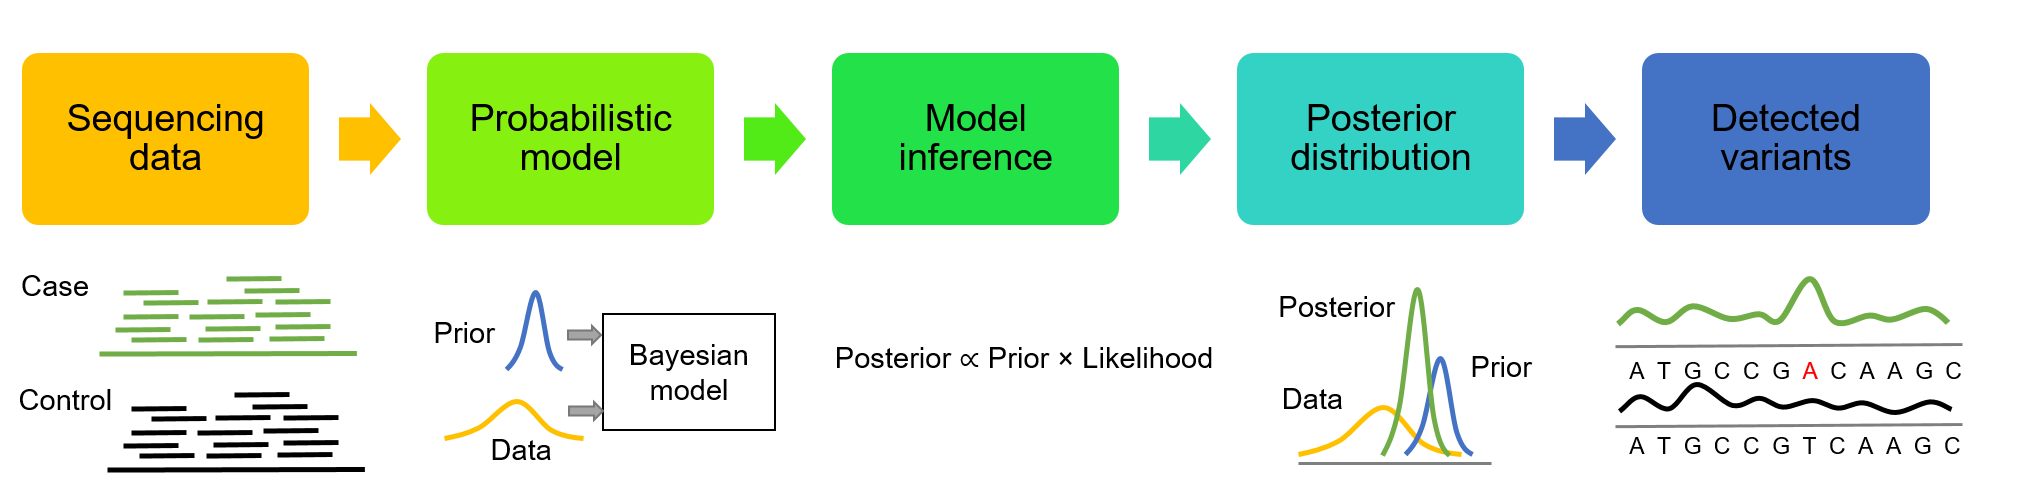
\includegraphics[width=1\textwidth]{bayesian.png}
\caption{Bayesian probabilistic framework for variant detection in NGS sequencing data.
The control sample is shown in black and the case sample is shown in red.
The posterior distribution (green) is propotional to the prior distribution (blue) and the likelihood of the data distribution (yellow).}
\label{fig:Bayesian}
\end{figure*}


\subsection{Non-probabilistic methods}

We summary 5 variant detection methods that are developed based on non-probabilistic or other combination methodologies.

\textbf{SNVer}~\citep{Wei2011} is a common and rare variant detection method for both individual and pooled sequencing data and it is scalable for whole genome sequencing data.
This is a frequentist method that reports overall P-values for every site without discarding bases with low read depth.
Transition/transversion ratio, genotype concordance, and dbSNP are metrics for evaluating the quality of variant calls in a real pooled sequencing data~\citep{depristo2011framework}.

\textbf{VarScan2}~\citep{Koboldt2012} is published for detecting somatic variants, loss of heterozygosity, and germline variants in exome sequencing data.
% "It also detects copy number variants but it is not related with our topic."
VarScan2 uses a heuristic method and a Fisher's exact test by comparing tumour and normal samples based on several thresholds, such as the number of allele counts and variant allele frequency.
In a test of 151 ovarian tumour samples from the TCGA data set, it identified 7,790 validated somatic variants with 93\% sensitivity and 85\% precision.

\textbf{Shimmer}~\citep{Hansen2013} is a method to identify somatic changes in normal-tumour samples.
It uses a Fisher's exact test with Benjamini-Hochberg~\citep{benjamini1995controlling} for multiple testing correction to control the false discovery rate (FDR).
Its advantage is that it is sensitive to detect variants in highly heterogeneous stromal contaminated data.

\textbf{Atlas2}~\citep{challis2012integrative} aims to detect SNVs in whole exome sequencing (WES) data from the platforms of SOLiD, Illumina, and Roche 454.
Atlas2 uses a logistic regression model to detect SNVs that pass several heuristic filters.
It has been integrated into the Genboree for easily processing the next-generation sequencing data on a web-based platform.

Feature-based classifiers~\citep{Ding2012}, such as random forests, Bayesian additive regression trees, support vector machines, and logistic regression, can also be used to detect somatic variants in tumour-normal paired data set.
Supervised machine learning algorithms are trained on the ground truth data set of $\sim 3400$ positions from $48$ breast cancer exome sequences and a cross-validation analysis is used to measure accuracy.
It shows that the feature-based machine learning algorithms outperform SAMtools and GATK in both sensitivity and specificity in this synthetic data set.

\textbf{Cake}~\citep{rashid2013cake} integrates four variant detection methods, Bambino, CaVEMan, SAMtools-mpileup, and VarScan2, together with post-processing filters to detect somatic variants.
Cake outperforms to any single algorithm with higher accuracy on two data sets, human hepatocellular carcinoma data and human breast cancer exome data.
It works well on WGS and WGE sequencing data by running on a standalone application.




\subsection{Overall Bayesian framework for variant detection}

Most of current variant detection methods are developed based on Bayesian Theorem. 
Here, we describe a overall workflow for developing Bayesian-based method for variant detection in Figure \ref{fig:Bayesian}.
First, control (normal sample) and case (tumour sample) sequencing data are commonly required to identify variants in the case.
Then, the control and case samples will be fed into a Bayesian probabilistic model independently for comparison. 
Besides the given data, a prior probabilistic distribution is needed to be defined for empirical Bayesian models.
The prior distribution captures the population knowledge of the parameters, like genotype information of the data, in the Bayesian statistical model.
Since the prior distribution affects the posterior distribution substantially, comparing posteriors under different plausible choices of prior distribution is important.
Once we have defined a model, the following work is model inference using Bayes' rule based on the prior and the likelihood of the data.
The posterior distribution is a compromise of the prior distribution and the data.
As an outcome of model inference, posterior distributions for control and case are obtained to detect variants.
%Finally, a hypothesis testing for comparison between the posterior distributions of control and case is conducted to reveal the point mutations with a significant difference between them.




\begin{landscape}
\begin{table}[htbp]
  \centering
  \small
  \caption{A summary of comparative analysis of variant detection methods.}\label{tbl:comparison}
  \begin{threeparttable}
    \begin{tabular}{rlrr}
    \multicolumn{1}{l}{\textbf{Benchmarking data sets}} & \textbf{Compared methods} & \multicolumn{1}{l}{\textbf{Advantages/Disadvantages}} & \multicolumn{1}{l}{\textbf{Ref}} \\
    \toprule
    \multicolumn{1}{l}{Illumina WES  CML} & VarScan & \multicolumn{1}{l}{Unable to detect rare variants of low VAFs.} &~\citep{Roberts2013} \\
          & JointSNVMix & \multicolumn{1}{l}{Vulnerable to FPs.} &  \\
          & SomaticSniper, Strelka & \multicolumn{1}{l}{Gave the best performance.} &  \\

    \midrule
    \multicolumn{1}{l}{Illumina WGS Melanoma } & VarScan2 & \multicolumn{1}{l}{Detected more somatic variants than others.} &~\citep{wang2013detecting} \\
    \multicolumn{1}{l}{Illumina WES lung tumour} & MuTect & \multicolumn{1}{l}{Detected most somatic variants of low VAFs.} &  \\
          & EBCall, JointSNVMix, Strelka, VarScan2 & \multicolumn{1}{l}{Had lower accuracy compared with VarScan2 and MuTect.} &  \\

    \midrule
    \multicolumn{1}{l}{Synthetic WGS} & GATK  & \multicolumn{1}{l}{Showed highest specificity and Ti/Tv ratio at single-sample. } &~\citep{liu2013variant}\\
          &       & \multicolumn{1}{l}{Showed higher sensitivity than SAMtools at multiple-sample.} &  \\
          & SAMtools, glftools, Atlas2 &       &  \\

    \midrule
    \multicolumn{1}{l}{Illumina WGS SSMP} & GATK, SAMtools & \multicolumn{1}{l}{Had the lowest FDR at 5$\times$ read depth.} &~\citep{Cheng2014}\\
    \multicolumn{1}{l}{with rare, low, and common VAFs} & CASAVA & \multicolumn{1}{l}{Had highest accuracy at 30$\times$ read depth.} &  \\
    \multicolumn{1}{l}{at 5$\times$, 10$\times$, 20$\times$, and 30$\times$ } & VarScan, glftools, SOAPsnp &       &  \\

    \midrule
    \multicolumn{1}{l}{Synthetic DNA mixtures } & SAMtools & \multicolumn{1}{l}{Had the lowest sensitivity.} &~\citep{Spencer2014}\\
    \multicolumn{1}{l}{with 2.5\% to 25\% VAFs at $>$ 1000$\times$ } & GATK,  SPLINTER & \multicolumn{1}{l}{Detected more than 94\% of variants with 10\% VAFs.} &  \\
          & VarScan2 & \multicolumn{1}{l}{Yielded more FPs at high read depths.} &  \\

    \midrule
    \multicolumn{1}{l}{WES with VAFs of 8\%, 16\%, 36\%, and 50\%} & MuTect, Strelka & \multicolumn{1}{l}{Showed highest sensitivity.} &~\citep{Xu2014}\\
    \multicolumn{1}{l}{Amplicon with VAFs of 8\%, 16\%, 36\%, and 100\%} & GATK, SomaticSniper, VarScan2 & \multicolumn{1}{l}{Sensitivity changed with VAFs.} &  \\

    \midrule
    \multicolumn{1}{l}{Synthetically pooled Illumina sequencing} & GATK, CRISP, LoFreq & \multicolumn{1}{l}{Showed 80\% accuracy with different read depths.} &~\citep{Huang2015} \\
          & VarScan, SNVer  & \multicolumn{1}{l}{Showed lower FPR but lower sensitivity.} &  \\
          
    \midrule
    \multicolumn{1}{l}{Breast cancer exome sequencing} & EBCall, MuTect, Virmid, Strelka & \multicolumn{1}{l}{Reported them to be the most reliable callers;} &~\citep{kroigaard2016evaluation} \\
    \multicolumn{1}{l}{Targeted deep sequencing} & & \multicolumn{1}{l}{Returned the lowest number of variants.} & \\
		&	& \multicolumn{1}{l}{EBCall and Mutect are robust to varying of read depth.} & \\
  		&  Shimmer, Somatic Sniper, VarScan2, Seurat & \multicolumn{1}{l}{Showed highly sensitive to increased depths;} &  \\
    		&	& \multicolumn{1}{l}{Returned high numbers of variants in low agreement with others.} & \\    
    		&	& \multicolumn{1}{l}{Seurat showed the highest sensitivity of $96\%$.} & \\            
        
    \bottomrule
    \end{tabular}
   \begin{tablenotes}
	\item The order of these methods are based on the published date.
CML, chronic myeloid leukemia;
WGS, whole genome sequencing;
FPs, false positives;
VAFs, variant allele frequencies;
FDR, false discovery rate;
WES, whole exame sequencing;
SSMP, Singapore sequencing malay project;
CASAVA, consensus assessment of sequence and variation;
Rare, VAF $<$ 1\%; Low, 1\% $\leqslant$ VAF $<$  5\%; common, VAF $\geqslant$ 5\%;
FPR, false positive rate;
Sensitivity, true positive rate;
Ti/Tv, transition/transversion ratio.
    \end{tablenotes}
\end{threeparttable}
\end{table}
\end{landscape}





A benefit of the Bayesian methods is the flexibility of multiple levels of random variables in measuring sources of uncertainty of underlying genotypes.
Bayesian framework has become a prevailing method to identify variants in the NGS data, but several difficulties still remain.
Computational calculation for Bayesian inference is normally difficult in the integration step.
Besides, accurate specification of prior probability in the model structure and model evaluation for fitness assessment are also challenging.




\subsection{Advantages and disadvantages of different methods}

Researchers are trying to compare performances of current variant detection methods in different applications based on their interests.
We summarize eight comparative analysis on variant detection methods in tumour-normal paired NGS data in Table \ref{tbl:comparison}.
The summary of method comparisons is helpful to select appropriate methods for their specific purposes.
These comparisons mostly focus on the performances of VarScan, MuTect, GATK, SAMtools, JointSNVMix, SomaticSniper, EBCall, and Strelka.
Synthetic or real WGS/WES data are used as benchmarking data sets for method validation.
Results of the comparative analysis show that SAMtools and GATK are not able to call rare variants in heterogeneous samples.
VarScan2 can detect more variants than other methods, but may yield more false positives~\citep{wang2013detecting, Spencer2014}.
Strelka returns a low number of variants in a conservative way~\citep{kroigaard2016evaluation}.
Although Strelka is able to call variants in heterogeneous samples, it has lower accuracy than MuTect~\citep{wang2013detecting}.
EBCall and MuTect are rubust to the changing of read depth and perform very well in a study of somatic variant detection in real exome and targeted deep sequencing data~\citep{kroigaard2016evaluation}.
Overall, MuTect outperforms other tested methods in detecting rare variants with low allele frequency and shows high sensitivity at different dilutions~\citep{wang2013detecting, Xu2014}.
Since the performance depends on the quality of specific data sets and the ability of methods in calling variants in heterogeneous samples, a combination of several state-of-the-art methods could be used together to generate an intersection of sets of the candidate variants for consistency~\citep{liu2013variant}.
A unified framework is provided for combining the detected variants from multiple variant detection methods with improved performance over each single method~\citep{kim2014combining}.


\subsection{The potential of deep learning in variant detection}

Recently, deep learning is active in solving computational biology problems and multiple layers of the deep networks will dissect the structure of high-throughput sequencing data~\citep{angermueller2016deep}.
Most current statistical methods are developed based on prior knowledge to analyze sequencing data.
For example, a prior probability was pre-defined for the allelic diversity for Snape~\citep{Raineri2012}.
In variant detection using SOAPsnp, the prior for homozygous variant rate is set as 0.0005 and for heterozygous rate is set as 0.001~\citep{Li2009}.
The prior probabilities were also set for both haploid and diploid genotypes according to the transition and transversion values in the study of dbSNPs alleles~\citep{zhao2002neighboring}. 
But, deep learning networks can learn directly from the data without assigning a prior.
A deep learning method, \textit{DeepBind}, is proposed to uncover the role of DNA/RNA binding proteins and also able to discover disease-related variants in sequencing data~\citep{alipanahi2015predicting}.
The advantage of deep learning methods is that it enabled direct training of the model on the sequencing samples.
Therefore, deep learning is very promising for variant detection to leverage a new direction for more accurate predictions.




\section{Conclusions}

This review addressed the necessity of sensitive variant detection methods and issues for rare SNVs detection in DNA NGS data.
We classified 30 state-of-the-art methods to different categories based on the methodology.
A Bayesian framework, as a leading method for current variant detection, is summarized for guidance of researchers to develop probabilistic statistical methods for variant detection.
It is expected that this review will help biologists and bioinformaticians in related fields to understand more about the current methods for rare variant detection and furthermore accelerate interpretation of the next-generation sequencing data for clinical studies. 


\subsection{Challenges and opportunities for statistical methods on rare variant detection}

A critical challenge for current statistical methods in rare variant detection is to reduce false positive calls.
It could be very easy for a statistical method to call a false positive when the allele frequency of a true positive variant is very close to the fraction of sequencing errors.
Increasing the depth of coverage may reduce false positive rate, but it is not guaranteed in all circumstances.
A possible solution is to estimate the pattern of sequencing errors as EBCall~\citep{Shiraishi2013} did to distinguish false positives from true rare variants.
Post-call filtering that consider parameters cut-offs may be also useful as VarScan2~\citep{Koboldt2012} did.

Another challenge is to improve the efficiency of statistical methods on whole genome-wide sequence analysis.
The size of whole-genome sequencing or whole-exome sequencing is large-scale and applications of them are being successfully integrated to the clinical diagnostics and development of precision medicine~\citep{chiang2012exome, worthey2011making}.
Inefficient variant detection in genome-wide sequencing data will definitely inhibit the effectiveness of translating the sequencing data into knowledge.
Computational parallelization can largely help to enhance efficiency by distribution of multiple computing cores, but there is room for improvement of scalability of statistical methods intrinsically.



\subsection{Perspectives}

Single nucleotide variant detection using statistical methods is an active area in the characterization of genomic heterogeneity in clinical samples.
A large number of statistical or computational methods have been developed for variant detection in the NGS data, but rare of them are applied to the cfDNA sequencing data.
As we have discussed, the biological and statistical issues that could hinder effective variant detection drive us to develop sensitively accurate, scalable, and robust methods.
Current methods have progressed quickly from the cut-off threshold methods, the genotypes subtraction methods, to the advanced Bayesian statistical methods.
Among these methods, the probabilistic statistical methods are built to handle uncertainty in the probabilistic analogues.
The un-probabilistic methods are embracing frequentist method, heuristic method, and other machine learning methods.
Each method has its own mathematical problem formulation and advantages and disadvantages.
Hence, accurate variant detection highly relies on the characteristics of the statisical methods.
Eventually, more sensitive statistical methods will continue to play a key part in the fundamental research on human genetics and the applications of cfDNA NGS data for clinical treatment. 








\section{Acknowledgments}
Funding




\subsubsection{Conflict of interest statement.} None declared.
\newpage

\bibliography{bib}
\bibliographystyle{plain}



\end{document}
